\documentclass[conference,a4paper]{IEEEtran}

% Escritura mejorada de fórmulas matemáticas
\usepackage{amsmath}

% Inserción de gráficos
\usepackage{graphicx}

% Escritura de pseudocódigo
\usepackage[kw]{pseudo}

% Escritura mejorada de tablas
\usepackage{booktabs}

% Escritura mejorada de citas bibliográficas
\usepackage{cite}

% Adicionales
\usepackage{hyperref}
\usepackage[framemethod=tikz]{mdframed}

% Macros traducidas
\def\contentsname{Índice general}
\def\listfigurename{Índice de figuras}
\def\listtablename{Índice de tablas}
\def\refname{Referencias}
\def\indexname{Índice alfabético}
\def\figurename{Fig.}
\def\tablename{TABLA}
\def\partname{Parte}
\def\appendixname{Apéndice}
\def\abstractname{Resumen}
% IEEE specific names
\def\IEEEkeywordsname{Palabras clave}
\def\IEEEproofname{Demostración}

\begin{document}

\newcounter{textb}[section] \setcounter{textb}{0}
\renewcommand{\thetextb}{\arabic{section}.\arabic{textb}}
\newenvironment{textb}[1][]{%
\refstepcounter{textb}%
\ifstrempty{#1}%
{\mdfsetup{%
frametitle={%
\tikz[baseline=(current bounding box)]
\node[rectangle,fill=white]
{\strut};}}%
}%
{\mdfsetup{%
frametitle={%
\tikz[baseline=(current bounding box)]
\node[rectangle, fill=black!10,draw=black] %<----------------------- added draw=black here
{\strut#1};}}% 
}%
\mdfsetup{innertopmargin=10pt, linecolor=black!80,%
linewidth=2pt,topline=true,%
frametitleaboveskip=\dimexpr-\ht\strutbox\relax
}
\begin{mdframed}[]\relax%
}{\end{mdframed}}


\title{
\includegraphics[scale=0.45]{figures/logo-us.png}\\Estudio de eficacia, capacidad, optimización y resultado del ensamblado de modelos de aprendizaje simples}

\author{
  \IEEEauthorblockN{Daniel Díaz Nogales}
  \IEEEauthorblockA{
    \textit{Dpto. Ciencias de la Computación e Inteligencia Artificial}\\
    \textit{Universidad de Sevilla}\\
    Sevilla, España\\
    UVUS: dandianog - Contacto: daniel0diiaz@gmail.com}
  
  \and
  
  \IEEEauthorblockN{Francisco Fernández Angulo}
  \IEEEauthorblockA{
    \textit{Dpto. Ciencias de la Computación e Inteligencia Artificial}\\
    \textit{Universidad de Sevilla}\\
    Sevilla, España\\
    UVUS: fraferang - Contacto: francsico.fer.an@gmail.com}
}

\maketitle


% Resumen
\begin{abstract}

  El objetivo principal del trabajo es la realización y estudio de modelos de aprendizaje supervisados formados a partir de la composición secuencial de otros modelos de aprendizaje. Se busca estudiar la eficacia del ensamble de diferentes modelos de aprendizaje simples en un mismo modelo cuya capacidad sea mayor. \\
  
  Durante el estudio se ha desarrollado un prototipo de ensamble de diferentes modelos de aprendizaje de tipo regresión, y se ha probado con diferentes conjuntos de datos proporcionados. Se comprueba que la capacidad predictiva del modelo de aprendizaje ensamblado disminuye o aumenta en función de la cantidad de modelos de aprendizaje simples que lo componen, además de otros hiperparámetros que podremos especificar para cada modelo de aprendizaje supervisado. \\ 

\end{abstract}


% Palabras claves
\begin{IEEEkeywords}
  modelo de aprendizaje supervisado, ensamble, arboles de decisión, regresión
\end{IEEEkeywords}


\section{Introducción}

Buscando desarrollar un \textbf{modelo de aprendizaje supervisado fuerte} \cite{b7}, y con el objetivo de aumentar el rendimiento de modelos de aprendizaje débiles, estudiamos en este proyecto cómo garantizar mejor resultado de predicción. Para ello, implementaremos \textbf{ensamblado de modelos de aprendizaje secuenciales}, que aumentará la capacidad del modelo final de entender conjuntos de datos más complejos y ofrecer mejores predicciones. \\

En los modelos de aprendizaje débiles, las predicciones normalmente no coinciden con el valor esperado aunque se aproximan (y es más frecuente a mayor aumente la complejidad del conjunto de datos). \textbf{Podemos reducir esta diferencia} entre los resultados reales y predictivos (a partir de ahora denominaremos \textit{residuo} a esta diferencia) \textbf{uniendo diferentes modelos de aprendizaje que aprendan a optimizar el residuo de un modelo anterior} para así lograr que cada nueva iteración devuelva el menor posible. \\

Los modelos de aprendizaje permiten satisfacer dos tipos de problemas: \textbf{problemas de clasificación}, donde la variable objetivo tiene valores discretos, o \textbf{problemas de regresión} \cite{b1}, donde la variable objetivo tiene un valor continuo. Nos centraremos en este último tipo de problemas en nuestro estudio. Además, se pueden utilizar diferentes tipos de modelo de aprendizaje de tipo regresión para el ensamble, e incluso combinarlos entre sí. Realizamos el estudio haciendo uso de diferentes modelos de aprendizaje, como el árbol de decisión o vecinos cercanos (\textit{knn})\cite{b5}. \\

El \textbf{ensamble de modelos de regresión} \cite{b2} propuesto funcionará sobre un conjunto de datos dado, donde se seleccionarán las \textbf{columnas atributos} y \textbf{columna objetivo}. Se dividirá dicho conjunto de datos en 2 partes, formando un \textbf{conjunto de entrenamiento} y un \textbf{conjunto de evaluación}. Se entrentará un primer modelo con el conjunto de entrenamiento, y devolverá una primera predicción inicial evaluada con una matriz de valores medios de cada columna del conjunto de datos. Nos permitirá obtener nuestro primer residuo, con el que podremos entrenar nuestro siguiente modelo secuenciando la creación de sub-modelos, que aprenderán sobre el cálculo del residuo del modelo anterior. \\

Finalmente nuestro ensamble \textbf{devolverá una lista de modelos entrenados y la predicción final}. Ésta la  utilizaremos para compararla con la predicción real y obtener una puntuación de calidad global.\\

La información del artículo ha sido clasificada en diferentes apartados. Una vez contextualizado el objeto de estudio, y la dinámica que seguirá el prototipo de ensamble propuesto, se profundiza más sobre cada concepto en los siguientes índices.


\section{Preliminares}

Se dispone de 3 conjuntos diferentes de datos \cite{b8, b9, b10} con los que se realizarán los experimentos en nuestro estudio. Son conjuntos de datos públicos, y consisten simplemente en columnas de atributos que nos servirán para entrenar nuestro ensamble de algoritmo, y una columna objetivo con las variables de respuesta. Los 3 conjuntos de datos utilizados se llaman \textbf{adultDataset}\cite{b8}, \textbf{titanic}\cite{b9} y \textbf{BreastCancerDataset}\cite{b10}.\\


\subsection{Métodos empleados}

Tras el estudio de los fundamentos de diferentes modelos de aprendizaje de regresión \cite{b5, b6, b15}, y los problemas de \textbf{tipo regresión} \cite{b1, b2}, planteamos el prototipo de forma simplificada como un problema dividido en 3 fases. \\

En la fase 1 se busca tener un primer modelo de aprendizaje entrenado con los conjuntos de datos proporcionados. Para ello, tendremos que elegir primero qué columnas serán los atributos de datos, y qué columna será la objetivo. Después, se preprocesará las columnas de atributos y objetivo con el fin de codificar\cite{b11, b12} los valores para que el algoritmo de aprendizaje del modelo pueda trabajar con ellos.\\

Con los datos codificados, \textbf{se dividen los conjuntos de atributos de datos y objetivos codificados en conjuntos de entrenamiento y de prueba} con el método \textit{train\_test\_split} \cite{b13}. \textbf{Se define el primer modelo de aprendizaje} de clase \textit{DecisionTreeRegressor} \cite{b2} o \textit{KNeighborRegressor}, que construye el árbol con el método \textit{fit} \cite{b16} a partir del conjunto de atributos y objetivo de la muestra de entrenamiento. \\

Se realiza la predicción con el método \textit{predict} \cite{b14} del modelo de aprendizaje seleccionado cuyo conjunto de evaluación serán los valores medios de todas las columnas del conjunto de datos. Esta primera predicción nos servirá para la fase 2, donde se comenzarán a calcular residuos y los sub-modelos entrenarán a partir de éste. \\

La fase 2 se centra en crear nuevos sub-modelos que aprendan del residuo de anteriores. Iteraremos un algoritmo de aprendizaje, a partir de ahora será llamado meta-algoritmo, tantas veces como modelos queramos secuenciar en nuestro prototipo de ensamblaje. Este meta-algoritmo primero calculará el residuo de la predicción del árbol anterior. Luego obtendrá una muestra aleatoria sin reemplazamiento del conjunto de evaluación (de proporción hiperparámetro sample\_size) y su correspondiente residuo. Estos se utilizarán para entrenar un nuevo sub-modelo de aprendizaje, con el que se evaluará en una predicción el conjunto de evaluación. \\

\begin{figure}[ht]
  \begin{center}
    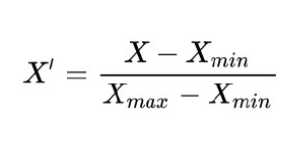
\includegraphics[scale=0.70]{figures/funcion_clasificacion_valores_prediccion.png}
    \caption{Clasificación de los valores de la predicción en el rango [Xmin, Xmax] para que pertenezcan a las clases 1 o 0}
    \label{fig:funcion_clasificacion}
  \end{center}
\end{figure}

En la fase 3 se busca recolectar los datos obtenidos por los modelos para poder estudiarlos. Del meta-algoritmo se obtiene una lista de árboles entrenados y una puntuación llamada \textit{BalancedAccuracyScore} \cite{b17}. Esta puntuación es creada a partir de la diferencia entre los valores reales del conjunto de evaluación y la predicción del último modelo, y nos dará una idea de la calidad predictora del ensamble de modelos. Como nuestra predicción no nos dará valores exactos, y necesitamos clasificar sus clases, aplicamos a la predicción el método classify\_prediction (sigue la función de clasificación del a figura \ref{fig:funcion_clasificacion}. Con esto ejecutaremos diferentes pruebas a los diferentes conjuntos de datos. La figura \ref{fig:nmodels_titanic} muestra la evolución de diferentes evaluaciones del ensamble cambiando la cantidad de modelos secuenciales.\\


\begin{figure}[ht]
  \begin{center}
    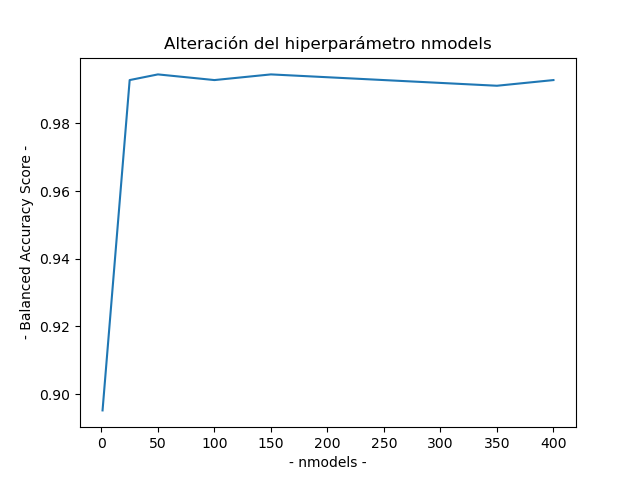
\includegraphics[scale=0.30]{figures/nmodels_titanic_tree.png}
    \caption{Diferentes BalancedAccuracyScores del ensamblado cambiando hiperparámetro nmodels en el conjunto de datos Titanic.}
    \label{fig:nmodels_titanic}
  \end{center}
\end{figure}


Dentro de los ejemplos del estudio, utilizamos las \textbf{funciones elementales de Python y numpy} \cite{b18} para condicionamiento y procesado de datos, la librería \textbf{matplotlib} \cite{b19} para diferentes gráficas, varios \textbf{métodos de librerías de sklearn} \cite{b1, b2, b3, b4, b11, b12, b13, b14, b15, b16, b17} para la definición de clases de modelos de aprendizaje y desarrollo, \textbf{pandas} \cite{b20} para el trabajo de ficheros. \\


\section{Metodología}

Se han preparado dos clases en dos ficheros externos que son importados como módulo. Dicha clase se construye con los hiperparámetros del problema, y se ejecuta con su método start(X, y), cuyos parámetros son los conjuntos de datos de un dataset. Se explica la metolodología detalladamente por fases tal y como el anterior apartado. \\

Antes de entrar en la fase 1, definiremos las columnas  de atributos y la columna objetivo que procesará nuestro ensamble. Se definirá un objeto de tipo \textit{SequencialModelAlgorithm} y se le pasarán los hiperparámetros de ejecución.

\begin{textb}[1. Constructor de SequencialModelAlgorithm]

\textbf{Entrada}:
    \begin{itemize}
    \item \textbf{nmodels}: número de modelos secuenciales
    \item \textbf{sample\_size}: proporción de datos a coger en la muestra sin reemplazamiento del meta-algoritmo
    \item \textbf{max\_depth}: profundidad en los árboles de decisión para devolver solución
    \item \textbf{lr}: factor de aprendizaje de los modelos secuenciales
    \item \textbf{min\_samples\_leaf}: mínimo de ejemplos por hoja en el modelo por árboles de decisión
    \item \textbf{max\_features}: número máximo de características a considerar
    \item \textbf{min\_weight\_fraction\_leaf}: fracción mínima ponderada de la suma total de pesos de las hojas
\end{itemize}
\textbf{Salida}:
\begin{itemize}
    \item Objeto de tipo SequencialModelAlgorithm
\end{itemize}
\textbf{Algoritmo}:
\begin{enumerate}
    \item Almacena los parámetros como atributos de la clase
\end{enumerate}
\end{textb}

Fijados estos parámetros, y entrando en la primera fase, se inicializa un método para comenzar el entrenamiento del primer modelo de aprendizaje y el meta-algoritmo. \\

\begin{textb}[2. Método start]

    \textbf{Entrada}:
    \begin{itemize}
    \item \textbf{attributes\_cols}: columnas de atributos del conjunto de datos
    \item \textbf{objetive\_col}: columna objetivo del conjunto de datos
    \item \textbf{random\_state}: semilla para la muestra del conjunto de datos
    \item \textbf{ftest\_size}: proporción para la división del primer conjunto de datos en conjunto de entrenamiento y de evaluación
\end{itemize}
\textbf{Salida}:
\begin{itemize}
    \item Conjunto de modelos de aprendizaje débiles entrenado
    \item Puntuación de calidad \textit{BalancedAccuracyScore}
\end{itemize}
\textbf{Algoritmo}:
\begin{enumerate}
    \item Preprocesado de atributos y codificación con método \textit{attributes\_preprocess}
    \item Preprocesado del objetivo y codificación con método \textit{objetive\_preproccess}
    \item División de los atributos y objetivo en conjunto de entrenamiento y evaluación
    \item Selección y definición del modelo de aprendizaje
    \item Entrenamiento del modelo de aprendizaje con el conjunto de entrenamiento
    \item Primera predicción evaluando el valor medio de las columnas de atributos
    \item Ejecutar \textit{nmodels} veces el método meta\_algorithm y acumular cada árbol
    \item Calcular la puntuación BalancedAccuracyScore de la última predicción con respecto a los datos de respuesta reales
\end{enumerate}
\end{textb}

Los submétodos utilizados en el método start para el preprocesado y codificación de las variables de los conjuntos de datos son: \\
\begin{textb}[3. Método attributes\_preprocess]

    \textbf{Entrada}:
    \begin{itemize}
    \item \textbf{attributes\_cols}: columnas de atributos
\end{itemize}
\textbf{Salida}:
\begin{itemize}
    \item Columnas de atributos preprocesadas y codificadas
\end{itemize}
\textbf{Algoritmo}:
\begin{enumerate}
    \item Para cada columna de atributos:
    \begin{enumerate}
      \item Leer el primer valor del primer índice de la columna
      \item Si el primer valor de la columna no es de tipo numérico:
        \begin{enumerate}
          \item Se codifica con el método \textit{OrdinalEncoder}
        \end{enumerate}
    \end{enumerate}
\end{enumerate}
\end{textb}

\begin{textb}[4. Método objetive\_preprocess]

    \textbf{Entrada}:
    \begin{itemize}
    \item \textbf{attributes\_cols}: columna de valores objetivo
\end{itemize}
\textbf{Salida}:
\begin{itemize}
    \item Columnas de valores objetivo preprocesadas y codificadas
\end{itemize}
\textbf{Algoritmo}:
\begin{enumerate}
    \item Leer el primer valor del primer índice de la columna
    \item Si el primer valor de la columna no es de tipo numérico:
      \begin{enumerate}
        \item Se codifica con el método \textit{LabelEncoder}
      \end{enumerate}
\end{enumerate}
\end{textb}

Finalmente dentro de la función start, tenemos el método \textbf{meta-algoritmo}, que recoge el aprendizaje de cada modelo secuencial, y el método classify\_prediction, que clasifica la respuesta del cómputo total de predicciones. Esto correspondería con las fase 2 de iteración del meta-algoritmo, y la fase 3 de evaluación de datos \\

\begin{textb}[5. Método meta\_algorithm]
    \textbf{Entrada}:
    \begin{itemize}
    \item \textbf{X}: columnas de valores atributo
    \item \textbf{y}: columna de valores objetivo
    \item \textbf{prediction}: predicción del modelo anterior
\end{itemize}
\textbf{Salida}:
\begin{itemize}
    \item Modelo de aprendizaje entrenado
    \item Predicción del nuevo modelo entrenado
\end{itemize}
\textbf{Algoritmo}:
\begin{enumerate}
    \item Calcula el residuo a partir de la diferencia de la columna objetivo y la predicción del anterior modelo
    \item Se recoge una muestra aleatoria de tamaño proporción sample\_size de los datos de atributos y objetivo
    \item Se define el modelo de aprendizaje con los hiperparámetros
    \item Se entrena el modelo con los datos de atributos y objetivo de la \textit{muestra sin reemplazamiento}
    \item Se realiza la predicción del actual modelo como la suma de la predicción anterior más la suma de la actual producto con el factor de aprendizaje \textit{lr}
\end{enumerate}
\end{textb}

\begin{textb}[6. classify\_prediction]
    \textbf{Entrada}:
    \begin{itemize}
    \item \textbf{pred}: predicción
\end{itemize}
\textbf{Salida}:
\begin{itemize}
    \item predicción con valores clasificados
\end{itemize}
\textbf{Algoritmo}:
\begin{enumerate}
    \item Calcula el valor máximo continuo que tiene la predicción
    \item Calcula el valor mínimo continuo que tiene la predicción
    \item Para cada índice de la predicción, realizamos la función de clasificado de la figura 2
\end{enumerate}
\end{textb}

Dentro del método meta-algoritmo se desarrollan los siguientes métodos:


\begin{textb}[7. sample\_without\_replacement]
    \textbf{Entrada}:
    \begin{itemize}
    \item \textbf{X}: conjunto de atributos de evaluación
    \item \textbf{res}: conjunto de residuos calculado
    \item \textbf{sample\_size}: proporción a tener en cuenta para la cantidad de muestra
\end{itemize}
\textbf{Salida}:
\begin{itemize}
    \item Muestra de atributos de proporción sample\_size
    \item Muestra de residuos de proporción sample\_size
\end{itemize}
\textbf{Algoritmo}:
\begin{enumerate}
    \item Calcula el valor máximo continuo que tiene la predicción
    \item Calcula el valor mínimo continuo que tiene la predicción
    \item Para cada índice de la predicción, realizamos la función de clasificado de la figura 2
\end{enumerate}
\end{textb}


\section{Resultados}

Se recogen diferentes resultados con diferentes pruebas y evaluaciones en los diferentes Dataset. Estas pruebas se evaluarán con los siguientes valores predeterminados:
\begin{itemize}
    \item nmodels = 300
    \item sample\_size = 0.65
    \item max\_depth = 10
    \item lr = 0.1
\end{itemize}
Se realizan las siguientes evaluaciones para cada conjunto de datos: \\
\begin{itemize}
\item Prueba en función de nmodels: realizamos la prueba fijando los parámetros predeterminados y variando nmodels entre diferentes valores dependiendo del dataset
\item Prueba en función de sample\_size: se fijan los hiperparámetros predeterminados y se altera sample\_size entre 0.1 y 0.9. Como influye poco en el resultado, y la aletoriedad es más fuerte que esta influencia del parámetro, se propone repetir 5 veces la prueba y devolver un valor medio entre las 5.
\item Prueba en función de max\_depth: se fijan los hiperparámetros predeterminados y se altera max\_depth entre 1 y 20
\item Prueba en función de lr: se fijan los hiperparámetros predeterminados y se altera lr entre 0.1 y 0.9. También se propone repetir 5 veces la prueba y devolver un valor medio entre las 5.
\item Prueba en función de nmodels utilizando Vecinos Cercanos: se fijan los hiperparámetros predeterminados y se altera nmodels entre 1 y 350.
\item Prueba en función de n\_neighbors utilizando Vecinos Cercanos: se fijan los hiperparámetros predeterminados y se altera n\_neighbors entre 1 y 5.
\end{itemize}

Además, según los datos obtenidos para estas diferentes pruebas, elegimos los valores que mejor determinen nuestro resultado de predicción en nuestro ensamble de modelos. Evaluaremos este resultado en función de los recursos que necesite el algoritmo, el tiempo de ejecución y la certeza en su solución. \\

Para ver cómo el algoritmo funciona según la complejidad de los conjuntos de datos proporcionados, se divide en subsecciones con diferentes comparaciones de las evaluaciones en los diferentes conjuntos de datos.

\subsection{Alteración del hiperparámetro nmodels}

Variaremos la cantidad de modelos de aprendizaje que ensamblan el prototipo propuesto, y lo aplicaremos a diferentes datasets con el fin de sacar conclusiones sobre cómo interfiere la cantidad de modelos aplicados según la complejidad del conjunto de datos.

\begin{textb}[1. nmodels en adultDataset Árboles de Decisión]
    \textbf{Hiperparámetros}:
  \begin{itemize}
      \item \textbf{nmodels} = [1, 50, 100, 150, 250, 350, 500]
      \item \textbf{sample\_size} = 0.65
      \item \textbf{max\_depth} = 10
      \item \textbf{lr} = 0.1
  \end{itemize}
  \textbf{Gráfico}
  
  \begin{center}
    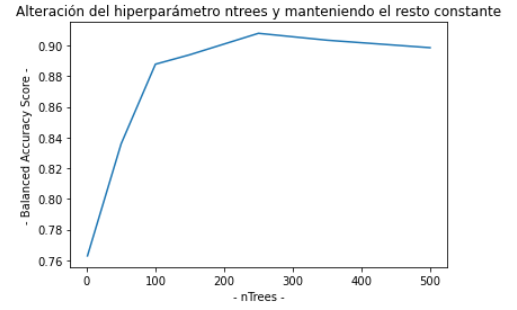
\includegraphics[scale=0.60]{figures/nmodels_adultDataset_tree.png}
    \label{fig:funcion_clasificacion}
  \end{center}
  
  \textbf{Comentarios} adultDataset necesita entre 200 y 250 modelos de aprendizaje secuenciales para devolver la mejor puntuación. Es una función logarítmica, por lo que intuimos que no obtendremos mucha mejor puntuación a cambio de más modelos. \\
  Por optimización podríamos decir que un buen valor para nmodels en adultDataset sería 250
\end{textb}

\begin{textb}[2. nmodels en titanic.csv por Árboles de Decisión]
    \textbf{Hiperparámetros}:
  \begin{itemize}
      \item \textbf{nmodels} = [1, 50, 100, 150, 250, 350, 500]
      \item \textbf{sample\_size} = 0.65
      \item \textbf{max\_depth} = 10
      \item \textbf{lr} = 0.1
  \end{itemize}
  \textbf{Gráfico}
  
  \begin{center}
    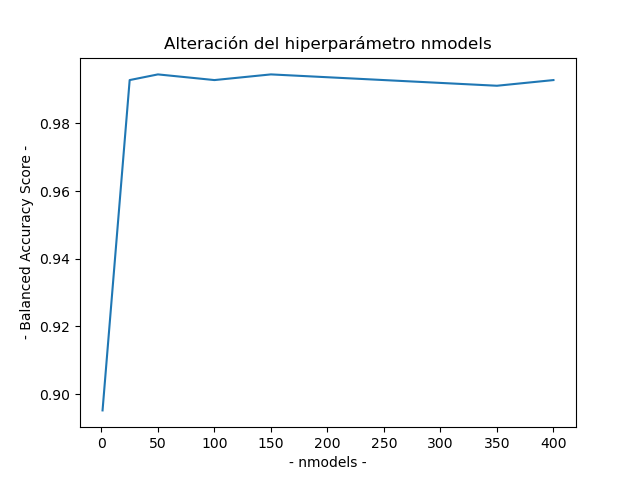
\includegraphics[scale=0.5]{figures/nmodels_titanic_tree.png}
    \label{fig:funcion_clasificacion}
  \end{center}
  
  \textbf{Comentarios} titanic necesita aproximadamente 50 modelos de aprendizaje secuenciales para devolver la mejor puntuación. Es función logarítmica aún más marcada que en el anterior dataset, por lo que intuimos que no obtendremos mucha mejor puntuación a cambio de más modelos. \\
  Por optimización podríamos decir que un buen valor para nmodels en titanic sería 50
\end{textb}

\begin{textb}[3. nmodels en BreastCancerDataset Árboles de Decisión]
    \textbf{Hiperparámetros}:
  \begin{itemize}
      \item \textbf{nmodels} = [1, 50, 100, 150, 250, 350, 500]
      \item \textbf{sample\_size} = 0.65
      \item \textbf{max\_depth} = 10
      \item \textbf{lr} = 0.1
  \end{itemize}
  \textbf{Gráfico}
  
  \begin{center}
    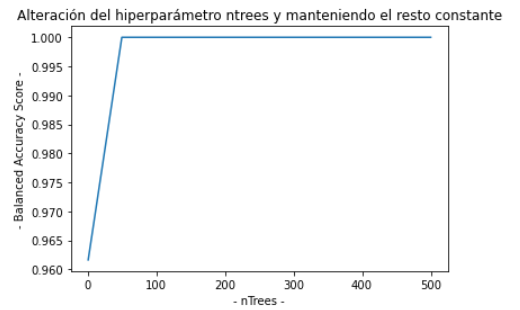
\includegraphics[scale=0.65]{figures/nmodels_BreastCancerDataset_trees.png}
    \label{fig:funcion_clasificacion}
  \end{center}
  
  \textbf{Comentarios} BreastCancer necesita 50 modelos de aprendizaje secuenciales para converger en una puntuación de predicción máxima en 1. Por optimización podríamos decir que un buen valor para nmodels en titanic sería 50
\end{textb}

Se repite el experimento haciendo uso de modelos de aprendizaje por vecinos más cercanos. Estas ejecuciones son mucho más largas según la cantidad de modelos en modelos más complejos como AdultDataset que usando árboles de decisión. 

Por consecuente, para AdultDataset se limita nmodels a un máximo de 25 modelos, mientras que en el conjunto titanic o BreastCancer llegaremos a 350 modelos.

\begin{textb}[4. nmodels en adultDataset Vecinos Cercanos]
    \textbf{Hiperparámetros}:
  \begin{itemize}
      \item \textbf{nmodels} = [1, 5, 10, 15, 20, 25]
      \item \textbf{n\_neighbors} = 1
  \end{itemize}
  \textbf{Gráfico}
  
  \begin{center}
    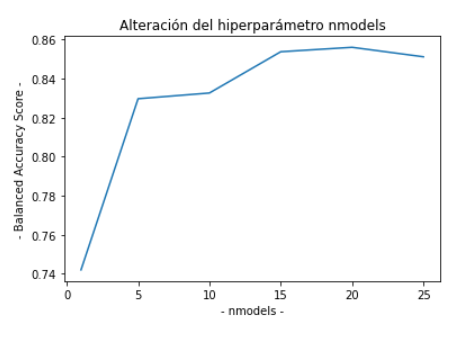
\includegraphics[scale=0.70]{figures/nmodels_adultDataset_knn.png}
    \label{fig:funcion_clasificacion}
  \end{center}
  
  \textbf{Comentarios} No podemos confirmar una función logarítmica en el modelo de aprendizaje por vecinos cercanos, pero la ejecución es mucho más lenta y aumenta según la cantidad de modelos de forma exponencial.
\end{textb}

La base de datos titanic tiene menor complejidad, por lo que nos permite hacer ejecuciones según nmodels menos pesadas. \\

\begin{textb}[5. nmodels en titanic Vecinos Cercanos]
    \textbf{Hiperparámetros}:
  \begin{itemize}
      \item \textbf{nmodels} = [1, 5, 10, 15, 20, 30, 50, 100, 175, 250, 350]
      \item \textbf{n\_neighbors} = 1
  \end{itemize}
  \textbf{Gráfico}
  
  \begin{center}
    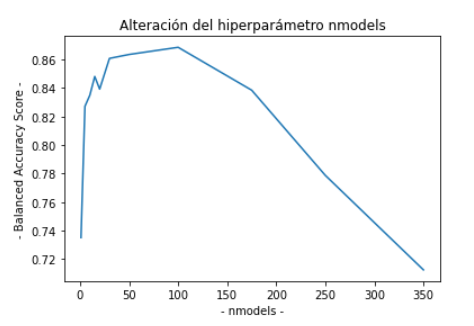
\includegraphics[scale=0.80]{figures/nmodels_titanic_knn.png}
    \label{fig:funcion_clasificacion}
  \end{center}
  
  \textbf{Comentarios} La función nos muestra que el valor óptimo de modelos de aprendizaje secuenciales estaría entre 50 y 100. Llega un momento en el que cuanto más modelos peor resultado.
\end{textb}

\begin{textb}[6. nmodels en BreastCancerDataset Vecinos Cercanos]
    \textbf{Hiperparámetros}:
  \begin{itemize}
      \item \textbf{nmodels} = [1, 5, 10, 15, 20, 30, 50, 100, 175, 250, 350]
      \item \textbf{n\_neighbors} = 1
  \end{itemize}
  \textbf{Gráfico}
  
  \begin{center}
    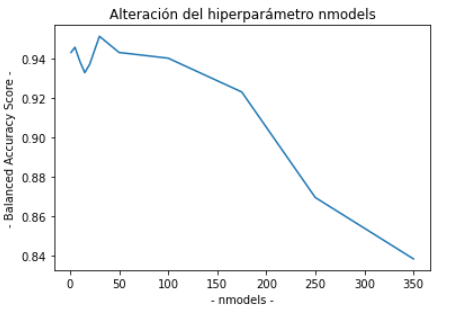
\includegraphics[scale=0.80]{figures/nmodels_BreastCancerDataset_knn.png}
    \label{fig:funcion_clasificacion}
  \end{center}
  
  \textbf{Comentarios} La función nos muestra que el valor óptimo de modelos de aprendizaje secuenciales estaría entre 50 y 100. Llega un momento en el que cuanto más modelos peor resultado.
\end{textb}

\subsection{Alteración del hiperparámetro sample\_size}

Se modifica la proporción de muestra que se utiliza para entrenar cada submodelo de aprendizaje secuencial. Estas pruebas se realizan 5 veces para mostrar en gráfica una media de los resultados con la intención de reducir el impacto que provocan resultados influidos por la aletoriedad.

\begin{textb}[7. sample\_size en adultDataset Árboles de Decisión]
    \textbf{Hiperparámetros}:
  \begin{itemize}
      \item \textbf{nmodels} = 300
      \item \textbf{sample\_size} = [0.1, 0.25, 0.5, 0.75, 0.9]
      \item \textbf{max\_depth} = 10
      \item \textbf{lr} = 0.1
  \end{itemize}
  \textbf{Gráfico}
  
  \begin{center}
    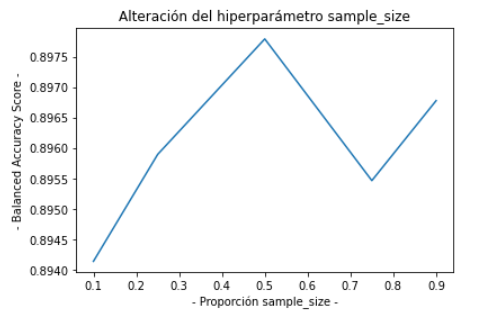
\includegraphics[scale=0.80]{figures/samplesize_adultDataset_trees.png}
    \label{fig:funcion_clasificacion}
  \end{center}
  
  \textbf{Comentarios} La proporción de la muestra óptima está en 0.5
\end{textb}

\begin{textb}[8. sample\_size en titanic Árboles de Decisión]
    \textbf{Hiperparámetros}:
  \begin{itemize}
      \item \textbf{nmodels} = 300
      \item \textbf{sample\_size} = [0.1, 0.25, 0.5, 0.75, 0.9]
      \item \textbf{max\_depth} = 10
      \item \textbf{lr} = 0.1
  \end{itemize}
  \textbf{Gráfico}
  
  \begin{center}
    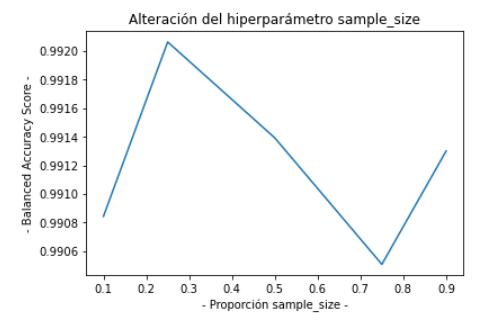
\includegraphics[scale=0.65]{figures/samplesize_titanic_trees.png}
    \label{fig:funcion_clasificacion}
  \end{center}
  
  \textbf{Comentarios} La proporción óptima de la muestra está en 0.2
\end{textb}

\begin{textb}[9. sample\_size en BreastCancer Árboles de Decisión]
    \textbf{Hiperparámetros}:
  \begin{itemize}
      \item \textbf{nmodels} = 300
      \item \textbf{sample\_size} = [0.1, 0.25, 0.5, 0.75, 0.9]
      \item \textbf{max\_depth} = 10
      \item \textbf{lr} = 0.1
  \end{itemize}
  \textbf{Gráfico}
  
  \begin{center}
    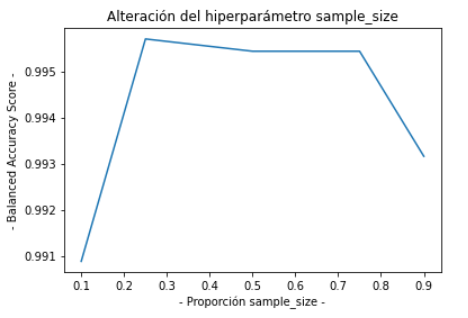
\includegraphics[scale=0.80]{figures/samplesize_BreastCancerDataset_trees.png}
    \label{fig:funcion_clasificacion}
  \end{center}
  
  \textbf{Comentarios} La proporción óptima de la muestra está entre 0.2 y 0.8
\end{textb}

\subsection{Alteración del hiperparámetro max\_depth}
Cambia la profundidad en la que se recorren los árboles de decisión. Esto será muy influyente en el resultado ya que precisa mayores soluciónes por modelo de aprendizaje aunque hace el proceso más pesado.

\begin{textb}[10. max\_depth en adultDataset Árboles de Decisión]
    \textbf{Hiperparámetros}:
  \begin{itemize}
      \item \textbf{nmodels} = 300
      \item \textbf{sample\_size} = 0.65
      \item \textbf{max\_depth} = [1, 5, 10, 15, 20]
      \item \textbf{lr} = 0.1
  \end{itemize}
  \textbf{Gráfico}
  
  \begin{center}
    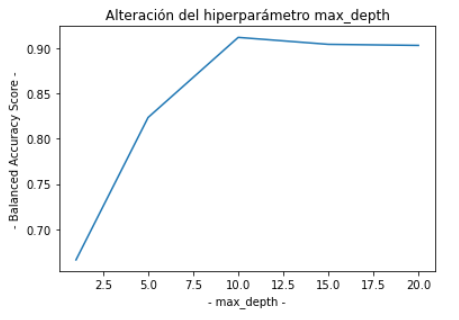
\includegraphics[scale=0.80]{figures/maxdepth_adultDataset_trees.png}
    \label{fig:funcion_clasificacion}
  \end{center}
  
  \textbf{Comentarios} El valor óptimo para el parámetro para la profundidad de árboles, max\_depth, es 10.
\end{textb}

\begin{textb}[11. max\_depth en titanic Árboles de Decisión]
    \textbf{Hiperparámetros}:
  \begin{itemize}
      \item \textbf{nmodels} = 300
      \item \textbf{sample\_size} = 0.65
      \item \textbf{max\_depth} = [1, 5, 10, 15, 20]
      \item \textbf{lr} = 0.1
  \end{itemize}
  \textbf{Gráfico}
  
  \begin{center}
    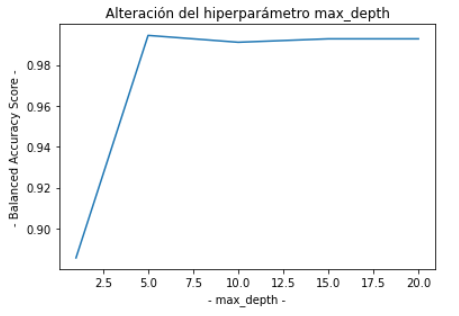
\includegraphics[scale=0.80]{figures/maxdepth_titanic_trees.png}
    \label{fig:funcion_clasificacion}
  \end{center}
  
  \textbf{Comentarios} El valor óptimo para el parámetro para la profundidad de árboles, max\_depth, es 5.
\end{textb}

\begin{textb}[12. max\_depth en BreastCancer Árboles de Decisión]
    \textbf{Hiperparámetros}:
  \begin{itemize}
      \item \textbf{nmodels} = 300
      \item \textbf{sample\_size} = 0.65
      \item \textbf{max\_depth} = [1, 5, 10, 15, 20]
      \item \textbf{lr} = 0.1
  \end{itemize}
  \textbf{Gráfico}
  
  \begin{center}
    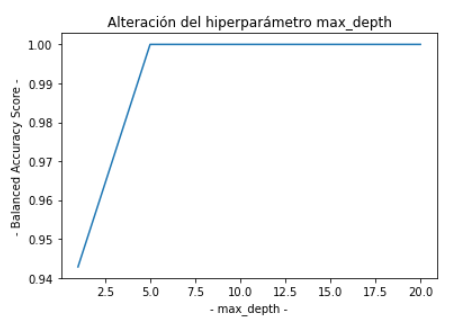
\includegraphics[scale=0.80]{figures/maxdepth_BreastCancerDataset_trees.png}
    \label{fig:funcion_clasificacion}
  \end{center}
\end{textb}

\subsection{Alteración del hiperparámetro ir}
Se altera el valor de la proporción o factor de aprendizaje. Estas pruebas se realizan 5 veces para mostrar en gráfica una media de los resultados con la intención de reducir el impacto que provocan resultados influidos por la aletoriedad.

\begin{textb}[13. max\_depth en adultDataset Árboles de Decisión]
    \textbf{Hiperparámetros}:
  \begin{itemize}
      \item \textbf{nmodels} = 300
      \item \textbf{sample\_size} = 0.65
      \item \textbf{max\_depth} = [1, 5, 10, 15, 20]
      \item \textbf{lr} = 0.1
  \end{itemize}
  \textbf{Gráfico}
  
  \begin{center}
    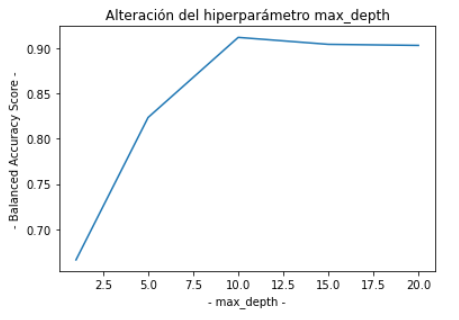
\includegraphics[scale=0.80]{figures/maxdepth_adultDataset_trees.png}
    \label{fig:funcion_clasificacion}
  \end{center}
  
  \textbf{Comentarios} El valor óptimo para el parámetro para la profundidad de árboles, max\_depth, es 10.
\end{textb}

\begin{textb}[14. lr en adultDataset Árboles de Decisión]
    \textbf{Hiperparámetros}:
  \begin{itemize}
      \item \textbf{nmodels} = 300
      \item \textbf{sample\_size} = 0.65
      \item \textbf{max\_depth} = 10
      \item \textbf{lr} = [0.1, 0.25, 0.5, 0.75, 0.9]
  \end{itemize}
  \textbf{Gráfico}
  
  \begin{center}
    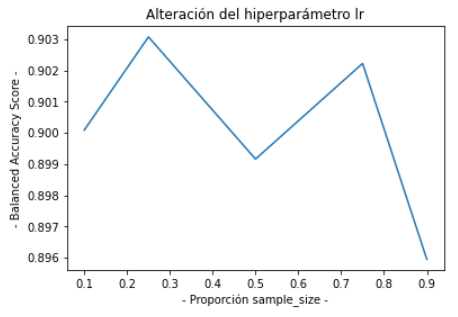
\includegraphics[scale=0.80]{figures/lr_adultDataset_trees.png}
    \label{fig:funcion_clasificacion}
  \end{center}
  
  \textbf{Comentarios} Aunque influye mucho la aletoriedad sobre el ejemplo, el valor medio mejor evaluado sería 0.2 como factor de aprendizaje
\end{textb}

\begin{textb}[15. lr en titanic Árboles de Decisión]
    \textbf{Hiperparámetros}:
  \begin{itemize}
      \item \textbf{nmodels} = 300
      \item \textbf{sample\_size} = 0.65
      \item \textbf{max\_depth} = 10
      \item \textbf{lr} = [0.1, 0.25, 0.5, 0.75, 0.9]
  \end{itemize}
  \textbf{Gráfico}
  
  \begin{center}
    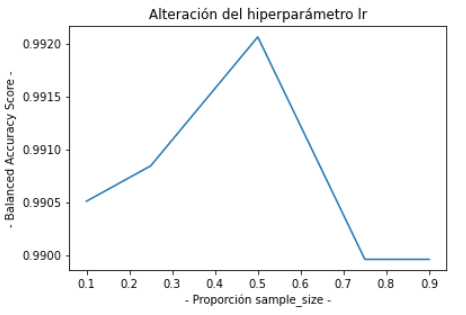
\includegraphics[scale=0.80]{figures/lr_titanic_trees.png}
    \label{fig:funcion_clasificacion}
  \end{center}
  
  \textbf{Comentarios} Aunque influye mucho la aletoriedad sobre el ejemplo, el valor medio mejor evaluado sería 0.2 como factor de aprendizaje
\end{textb}

\begin{textb}[16. lr en BreadCancerDataset Árboles de Decisión]
    \textbf{Hiperparámetros}:
  \begin{itemize}
      \item \textbf{nmodels} = 300
      \item \textbf{sample\_size} = 0.65
      \item \textbf{max\_depth} = 10
      \item \textbf{lr} = [0.1, 0.25, 0.5, 0.75, 0.9]
  \end{itemize}
  \textbf{Gráfico}
  
  \begin{center}
    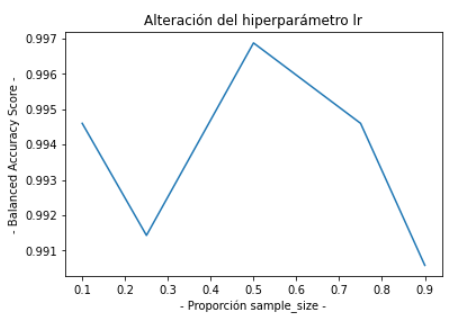
\includegraphics[scale=0.80]{figures/lr_BreastCancerDataset_trees.png}
    \label{fig:funcion_clasificacion}
  \end{center}
  
  \textbf{Comentarios} Aunque influye mucho la aletoriedad sobre el ejemplo, el valor medio mejor evaluado sería 0.5 como factor de aprendizaje
\end{textb}


\subsection{Exploración de otros hiperparámetros}

Se han implementado pruebas para otros hiperparámetros en los árboles de decisión y vecinos cercanos en las pruebas del prototipo en forma de cuaderno Jupyter.


\section{Conclusiones}

Tras el estudio concluimos que el ensamble de modelos de aprendizaje influye directamente en la calidad de predicción, tomando como valor de puntuación \textbf{BalancedAccuracyScore}. \\

El ensamble de modelos permite evaluaciones certeras en conjuntos de datos más complejos, como en \textit{AdultDataset} donde llegamos a una puntuación de 0.92 con la secuenciación de 250 árboles de decisión frente a los 0.68 que resuelve un solo árbol de decisión. Además, en conjuntos de datos menos complejos como \textit{titanic} o \textit{BreastCancer}, conseguimos con apenas 50 secuenciaciones puntuaciones de 0.99 o incluso 1. \\

Experimentando con los hiperparámetros, se concluye primero que influimos en la puntuación de calidad en función logarítmica a nmodels y max\_depth. Además son los parámetros con ajuste más preciso, se entiende fácilmente qué valor es mejor asignar a nuestro ensamble. Con el factor de aprendizaje, pero aún más con sample\_size, tenemos ejemplos muy influidos por la aletoriedad del experimento, por lo que hemos tratado de hacer la prueba varias veces y recoger los valores medios que devuelva. Aún así no se aprecia una función de influencia tan directa en la predicción del algoritmo de aprendizaje. \\


\begin{thebibliography}{00}
\bibitem{b1} Regresión en modelos de aprendizaje con sklearn \url{https://scikit-learn.org/stable/modules/svm.html#regression}
\bibitem{b2} Árboles de decisión con Regresión en sklearn \url{https://scikit-learn.org/stable/modules/generated/sklearn.tree.DecisionTreeRegressor.html}
\bibitem{b3} Método Shuffle de sklearn \url{https://scikit-learn.org/stable/modules/generated/sklearn.utils.shuffle.html}
\bibitem{b4} Función ColumnTransformer de sklearn \urn{https://scikit-learn.org/stable/modules/generated/sklearn.compose.ColumnTransformer.html}
\bibitem{b5} Árboles de decisión \url{https://www.cs.us.es/cursos/rac-2018/temas/tema-05.pdf}
\bibitem{b6} Árboles de decisión y algoritmo CART \url{https://www.uv.es/mlejarza/actuariales/tam/arbolesdecision.pdf}
\bibitem{b7} Modelos de aprendizajes fuertemente aprendedores vs modelos de aprendizajes débilmente aprendedores por ensamble \url{https://machinelearningmastery.com/strong-learners-vs-weak-learners-for-ensemble-learning/}
\bibitem{b8} Conjunto de datos AdultsDataset \url{https://archive.ics.uci.edu/ml/datasets/adult}
\bibitem{b9} Conjunto de datos titanic \url{https://www.kaggle.com/c/titanic}
\bibitem{b10} Conjunto de datos AdultsDataset \url{https://archive.ics.uci.edu/ml/datasets/adult}
\bibitem{b11} Codificación de objetivo LabelEncoder \url{https://scikit-learn.org/stable/modules/generated/sklearn.preprocessing.LabelEncoder.html}
\bibitem{b12} Codificación de atributo \url{https://scikit-learn.org/stable/modules/generated/sklearn.preprocessing.OrdinalEncoder.html}
\bibitem{b13} Separación de conjunto de entrenamiento y de prueba en sklearn \url{https://scikit-learn.org/stable/modules/generated/sklearn.model_selection.train_test_split.html}
\bibitem{b14} Método predict de Árboles de Decisión de tipo Regresión \url{https://scikit-learn.org/stable/modules/generated/sklearn.tree.DecisionTreeRegressor.html#sklearn.tree.DecisionTreeRegressor.predict}
\bibitem{b15} Vecinos cercanos con Regresión \url{https://scikit-learn.org/stable/modules/generated/sklearn.neighbors.KNeighborsRegressor.html}
\bibitem{b16} Métodos fit \url{https://scikit-learn.org/stable/modules/generated/sklearn.tree.DecisionTreeRegressor.html#sklearn.tree.DecisionTreeRegressor.fit} \url{https://scikit-learn.org/stable/modules/generated/sklearn.neighbors.KNeighborsRegressor.html#sklearn.neighbors.KNeighborsRegressor.fit}
\bibitem{b17} Balanced Accuracy Score \url{https://scikit-learn.org/stable/modules/generated/sklearn.metrics.balanced_accuracy_score.html}
\bibitem{b18} Numpy \url{https://numpy.org/}
\bibitem{b19} Simple graphic plot with matplotlib.pyplot \url{https://jakevdp.github.io/PythonDataScienceHandbook/04.01-simple-line-plots.html}
\bibitem{b20} 10 Minutes Pandas \url{https://pandas.pydata.org/pandas-docs/stable/user_guide/10min.html}
\end{thebibliography}


\end{document}
